\chapter{Gestión de Proyectos}

Scrum puede verse como un marco ágil de gestión de proyectos para el desarrollo incremental de productos, valiéndose de equipos autoorganizados. 



\subsection{Proyecto Scrum}

Un proyecto, en ingeniería de software, es un esfuerzo temporal que se lleva a cabo para crear un sistema, software o resultado único\footnote{Se parafrasea la definición del PMBOOK \cite{PMBOK-2004}.}. Los proyectos son organizados, en una empresa u organización, por el proceso de administración de proyectos. Según este proceso, el ciclo de vida de los proyectos se puede dividir en tres fases: inicio, ejecución y cierre (ver figura \ref{fig:PMIProject}). 

\subsection{Planificación}

En la administración de proyectos es necesario planificar y dicha actividad se suele hacer en la fase de inicio ("Starting phase" o "Project Start"). Pero, a diferencia de la metodología clásica (ver figura \ref{fig:PMIProject}) en que la planificación estaba siempre al inicio y el desarrollo en la fase de ejecución, en el marco Scrum la planificación se distribuye durante todo el ciclo de vida del proyecto y en la fase de ejecución se hace el desarrollo incremental de productos (por incrementos de producto) en iteraciones cortas (Sprint) donde cada iteración tiene su respectiva planificación (ver figura \ref{fig:ScrumProject}) y su incremento de producto, en caso de haberlo logrado (idealmente producto integrado y funcionando de cara al usuario o cliente).

\begin{figure}[h]
  \centering
  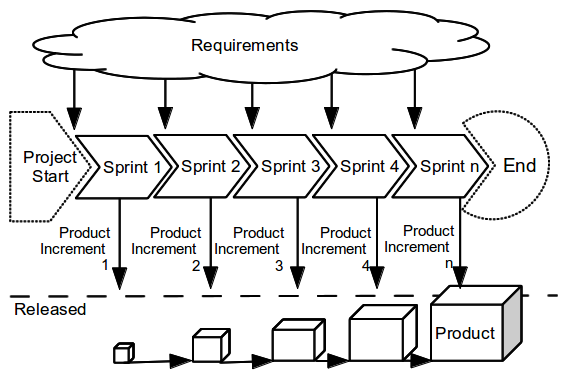
\includegraphics[width=0.90\textwidth]{ScrumProject}
  \caption{Proyecto Scrum}
  \centering
  \label{fig:ScrumProject} %\ref{fig:ScrumProject}
\end{figure}

Entonces podemos decir que en Scrum se piensa en muchos planes periódicos (a corto plazo). Los mismo pueden estar en un plan mayor a largo plazo pero de carácter flexible. También se puede realizar un plan global de entregables en base a los incrementos de producto estimados. Pero, desde esta perspectiva, hay que considerar que aunque se trabaje con planificaciones, los planes no son contratos a respetar a rajatabla.

\subsubsection{Inicio de proyecto}

En la etapa de inicio de proyecto ("Project Start") se puede hacer una “inception”, aunque esta técnica no es parte de Scrum. En una inception se hace un plan versátil alto nivel a corto plazo (un roadmap o release plan) para poder guiar e iniciar el desarrollo bajo el esquema Scrum.

%Triangle of Project Management
\subsection{Triángulo de la Gestión de proyectos}

Bajo el marco de Scrum se cambia la idea relacionada al triángulo clásico de la gestión de proyectos (o triángulo de hierro). El compromiso ya no es entre el tiempo, presupuesto y calidad; sino que se basa en el triángulo de: presupuesto (costo), tiempo (agenda) y funcionalidad (alcance) (ver figura \ref{fig:ScrumProjectManagementTriangle}) \footnote{The iron triangle of planning, Atlassian, Tareq Aljaber, 2017.}. Además, tradicionalmente se ha intentado fijar el alcance para negociar y variar el presupuesto y el tiempo. En cambio, desde la perspectiva ágil, se intentan mantener fijos el tiempo y el presupuesto, mientras se varía el alcance\footnote{\cite{Martin-Alaimo-2014}}. Cuando consideramos el presupuesto fijo (costo del equipo), pretendemos mantener al equipo fijo (equipo estable). Pues se desea equipos estables que maduren, se fortalezcan y, en consecuencia, se transformen en equipos de alto rendimiento. Por otro lado, una manera de trabajar con tiempos fijos es que el equipo se comprometa a trabajar en iteraciones fijas (sprints). Además el equipo podría fijar releases o bloques temáticos dado un tiempo. Y esto no es trabajar bajo “deadlines”, ya que el enfoque no es trabajar orientados a fechas, sino a valor de negocio. Entonces nos queda el alcance, descompuesto en ítems de backlog, y la pregunta ahora es: ¿cuánto puedes hacer en este tiempo y bajo un costo fijo para alcanzar los objetivos de negocio?

\begin{figure}[h]
  \centering
  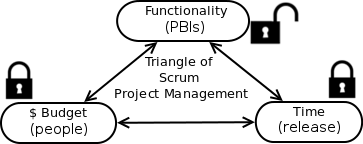
\includegraphics[width=0.60\textwidth]{ScrumProjectManagementTriangle}
  \caption{Triángulo de Gestión de Proyectos Scrum}
  \centering
  \label{fig:ScrumProjectManagementTriangle} %\ref{fig:ScrumProjectManagementTriangle}
\end{figure}

\subsubsection{Priorización trade-off}

La ventaja de esta aproximación es que en vez de focalizarnos en plazos con fechas de entrega, nos centramos en desarrollar valor. ¿Cual es el máximo valor que podemos desarrollar en un tiempo dado? Aquí entra el concepto de priorización trade-off, que se lleva a cabo en la ejecución del proyecto (o construcción de un producto). Trade-off es un acuerdo en el cual se deja algo fuera para priorizar otra cosa que se desea más. Pues, ante cambios, se prioriza un ítem reemplazando por otro de esfuerzo semejante para cumplir con entregar valor. Si en una iteración llega un cambio rompe fila, entonces vemos qué podemos sacar del sprint con mismo peso de esfuerzo. Lo mismo si queremos cumplir con un objetivo deseado en un tiempo planificado y necesitamos introducir un nuevo trabajo, pues revisaremos qué podemos sacar de esfuerzo semejante y cuyo valor podemos despriorizar en relación al cambio deseado.

Como vemos, aquí el enfoque viró rotundamente en relación a la administración clásica. En vez de asfixiar a los equipos para que lleguen a cumplir con una fecha, por lo general impuesta arbitrariamente, se les permite tener cierta autonomía (con un responsable de negocio) para que prioricen qué valor de negocio pueden entregar, para un objetivo planeado, con colaboración y participación del equipo mismo.

Bien, para que haya trade-off debe haber planificación. Pues siguiendo la disciplina de Scrum se planifica bastante. A continuación vemos este tema.


\subsection{Planificación de entregables}

Con este marco de trabajo tampoco es necesario hacer una entrega final (o "releasing") ya que se pueden hacer entregas paulatinas. En cada Sprint se puede entregar valor según lo planificado dentro del mismo sprint (planning). Además, para hacer diversas entregas intermedias planificadas se puede crear un plan de muy alto nivel para múltiples Sprints durante una planificación de lanzamientos (por ejemplo en una inception) llamado "Release Plan". Este plan de entregables o de lanzamientos es una guía con la que se pretende reflejar las expectativas sobre qué funcionalidad se implementará y cuándo, aproximadamente, se completará \footnote{\cite{Scrum-Institute-2015}}. También sirve como una base para monitorear el progreso dentro del proyecto. Pero siempre hay que considerar que no es un plan equivalente a un plan clásico, los hitos de releases no deberían ser compromisos rígidos y contractuales y, además, el desarrollo del proyecto no debería centrarse en respetar el plan. Por este motivo el plan de lanzamiento no es un plan estático o rígido; pues, se cambia durante todo el proyecto cuando nuevos requerimientos o conocimientos están disponible y, por ejemplo, cuando entradas PBIs en el Scrum Product Backlog cambian y se re-estiman. Por lo tanto, este plan debe ser revisado y actualizado colaborativamente en intervalos regulares, por ejemplo, después de cada Sprint (en refinamientos o reuniones acordadas).

\subsubsection{Release Plan Ágil}

Un "Release Plan" ágil es, normalmente, un conjunto de historias de usuario (o épicas) agrupadas por "releases" o versiones del producto que se ponen a disposición de los usuarios \footnote{Release plan, jmbeas, 2011; Agile Estimating and Planning, Mike Cohn}. En otras palabras, es una planificación a media distancia como una proyección hacia adelante en una serie de sprints \footnote{Release Planning, Retiring the Term but not the Technique, Mike Cohn, 2012.}. Esta planificación es algo valiosa de hacer cuando se usa el marco Scrum, pero no es requerido por el "núcleo Scrum" o el "Scrum originario" \footnote{Gone are Release Planning and the Release Burndown, Ralph Jocham and Henk Jan Huizer in Community Publications, Scrum.org, Saturday, October 01, 2011; Ken Schwaber and Jeff Sutherland Release Updated Scrum Guide, David Bulkin, Infoq.com on Jul 27, 2011}. Se puede utilizar Scrum con éxito sin necesidad de utilizar “Release Planning”.

Hay que remarcar que bajo el marco Scrum, si se hace un Release Plan, debería ser un documento minimalista (buscando el principio de simplicidad), pensado para MVPs (producto de mínimo valor) o entregas frecuentes (respetando el valor de software funcionando), abierto a modificaciones constantes (adaptabilidad y desarrollo evolutivo), consensuado con el equipo (transparencia) y desarrollado por el PO en colaboración con el cliente y con el equipo de desarrollo (priorizando la conversación y no la relación contractual).

Luego hay que tener en cuenta que para crearlo se deben tener disponibles las siguientes cosas:

\begin{enumerate}
\item Un Product Backlog priorizado y estimado.
\item La velocidad estimada del Equipo Scrum.
\item Las condiciones de satisfacción (metas para la agenda, el alcance, los recursos) o impacto deseado.
\end{enumerate}

\subsection{Gestión de proyecto orientada a producto}

El verdadero objetivo de Scrum es conseguir un producto mínimo viable o MVP en manos de los futuros clientes cuán rápido sea posible y obtener sus comentarios como feedback temprano\footnote{\cite{Jeff-Sutherland-2016}}. MVP es una estrategia para el aprendizaje de forma iterativa sobre sus clientes para poner a prueba las hipótesis fundamentales del negocio \footnote{\cite{Greg-Gehrich-2012}}. Es un incremento de producto, subconjunto del 20\% de features que representan parte del 80\% de valor\footnote{\cite{Jeff-Sutherland-2016}}. Las features del MVP representan conceptualmente al producto final completo y se prueba con un grupo de usuarios "early adopters". Las pruebas deben ser medibles y se hacen sobre las hipótesis fundamentales del producto como negocio.

Por otro lado hay otro concepto que se maneja en el ámbito de la agilidad, el MMP (Minimal Marketable Product). El MMP es el producto con el más pequeño posible conjunto de features y que crea la experiencia del usuario deseada, y por lo tanto puede ser comercializado y vendido, tempranamente, con éxito.

Resumidamente, la gestión de proyecto se orienta al producto y su ciclo de vida. Un producto puede evolucionar mediante una secuencia de releases, de los cuales algunos entregan valor directamente de cara al público. Después de una etapa de creatividad y prototipado (si el producto es nuevo y/o novedoso), tendremos uno o una secuencia de entregables MVPs hasta llegar a un MMP, que será el mínimo producto que se lanza al mercado como tal. De allí en adelante comienza el crecimiento en escalamiento (Growth) e incremento de funcionalidad hasta alcanzar una madurez (maturity), para finalmente constituir un producto final estable o commodity (ver fig. \ref{fig:product_evolution})\footnote{\cite{Greg-Gehrich-2012}}.

\begin{figure}[h]
  \centering
  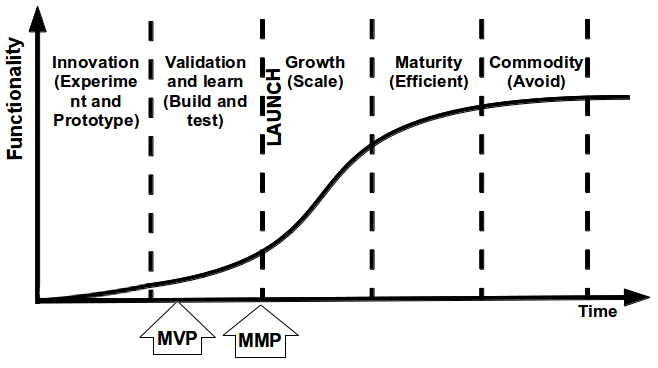
\includegraphics[width=0.70\textwidth]{product_evolution}
  \caption{Crecimiento del producto}
  \centering
  \label{fig:product_evolution} %\ref{fig:product_evolution}
\end{figure}

\subsubsection{Llevar trabajo a los equipos}

Al cambiar la perspectiva hacia estar orientados a productos y mantener equipos estables, cambia el enfoque de la gestión de proyectos. Ya no buscamos recursos humanos para proyectos, desarmando y armando equipos en función de proyectos. Lo que se busca hacer, entre otras cosas, es llevar trabajo a los equipos, buscando productos para equipos. Buscamos alinear a equipos en función de objetivos estratégicos. Mantener productos o servicios de valor para objetivos estratégicos. Donde los equipos son activos de la empresa y que buscan siempre maximizar el valor entregado. Esto puede llevar a cambiar toda la dinámica de funcionamiento de una PMO e, inclusive, desarrollar independientemente de presupuestos (tema que queda fuera del alcance de este libro).


\subsection{Gestión de riesgos}

Si bien la gestión de riesgos no es parte de scrum y un facilitador no se encarga de la gestión al modo tradicional como la gestión de riesgos, sí debería velar por mitigar los problemas que surjan en el proyecto y apoyar, en consecuencia, a la gestión de riesgos. En este sentido, no solo se encargaría de ayudar a desbloquear problemas y reducir impedimentos para que el sistema de trabajo fluya, sino que también puede preocuparse de prever issues para anticiparse a los problemas y controlar así, de antemano y en la medida de lo posible, los riesgos asociados a bloqueos del flujo de trabajo que atentan contra los objetivos del proyecto. Lo difícil es lograr una gestión de riesgos ágil en vez de una gestión pesada, dificultosa y que demande mucho esfuerzo de gestión. En esta vía, es preferible mantener un simple registro de riesgos con información concisa. Los datos principales a registrar de un riesgo, además de su nombre, pueden ser: descripción, probabilidad (probability), impacto (severity), criticidad (criticality), acciones de mitigación, dueño y estado.

Algo simple que se puede lograr trabajando con criticidad es usar tres valores en la probabilidad de ocurrencia y en el impacto (1, 2 y 3). El impacto representa la severidad de la ocurrencia de un problema asociado al riesgo o el tiempo perdido (size of loss). Por otro lado, la criticidad representa la prioridad del riesgo o el grado en que ese riesgo afecta negativamente al proyecto (exposure). El mismo será resultado del producto entre la probabilidad y el impacto. En consecuencia, la criticidad podría ser: 1, 2, 3, 4, 6, 9.

\begin{figure}[h]
  \centering
  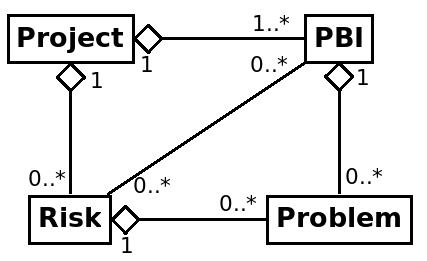
\includegraphics[width=0.40\textwidth]{RiskProblemDiagram}
  \caption{Diagrama de riesgos, problemas e ítems del proyecto (PBIs).}
  \centering
  \label{fig:RiskProblemDiagram} %\ref{fig:RiskProblemDiagram}
\end{figure}

Las herramientas gráficas que se pueden usar para dar visibilidad de los riesgos son: a) la “matriz de riesgos”; b) el “histórico de criticidad”; c) o el gráfico de curva de riesgo quemado (Risk Burn-down Chart).

La gestión de riesgos no es independiente de la gestión de impedimento o de problemas (issues o problem). Muchos de los problemas surgidos en el proyecto están asociados a riesgos identificados. Por tal motivo, la gestión de riesgos es útil, porque podemos mitigar los problemas de antemano. Por dicha razón, puede ser valioso llevar un registro de los issues y su relación con los riesgos. Siempre sin perder de vista no caer en el énfasis de la documentación ni en el afán de reportar. Se debe buscar la simplicidad y el foco en el flujo de trabajo sin impedimentos.

\begin{figure}[h]
  \centering
  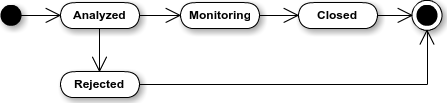
\includegraphics[width=0.70\textwidth]{RiskFlowDiagram}
  \caption{Estados posibles de un riesgo.}
  \centering
  \label{fig:RiskFlowDiagram} %\ref{fig:RiskFlowDiagram}
\end{figure}

Las herramientas gráficas útiles para dicha gestión son: “Tablero de Obstáculos” (obstacle board) o el "Calendario de Obstáculos" (Issues calendars).
